% !TeX spellcheck = fr_FR
\documentclass[11pt,a4paper,oneside]{report}
\usepackage[hmargin={1.25in,1.25in},vmargin={3cm,3cm}]{geometry}
%%%%%%%%%%%%%%%%%%%%%%%%
\setlength{\parindent}{0cm}
\makeindex
\usepackage{textcomp}
\usepackage{fancyhdr}
\usepackage{makeidx}
\pagestyle{myheadings}
\fancyhf{}
\rhead[\leftmark]{thepage}
%%%%%%%%%%%%%%%%%%%%%%%%

%\usepackage{natbib}
\usepackage[utf8]{inputenc}
\usepackage[T1]{fontenc} % pour taper les lettres accentuées
%\usepackage{charter} % change font style
%\usepackage[sc]{mathpazo}
\usepackage{utopia}
\usepackage{todonotes}
\usepackage[francais,english]{babel}
\usepackage{url}
\usepackage{graphicx}
\usepackage{breakurl}% si les refs dans la doc sont trop longues
\usepackage[bookmarks,bookmarksnumbered,citecolor=purple,colorlinks,hyperindex,linkcolor=black,linktocpage,urlcolor=ColorLink]{hyperref}
\usepackage{tikz}
\usepackage{pgfgantt} %draw timechart
\usepackage{amssymb, bm}
\newtheorem{mydef}{Définition}
\newtheorem{mytheorem}{Théorème}
\newtheorem{mylemme}{Lemme}

%\let\oldprintbibliography\printbibliography
%\renewcommand{\printbibliography}[1]{%
%  \let\chapter\section
%  \oldprintbibliography{#1}}

%\let\oldlistoftheorems\listoftheorems
%\renewcommand{\listoftheorems}[1]{%
%  \let\chapter\section
%  \oldlistoftheorems[#1]}

%\newcommand{\printsectionindex}{%
%  \let\chapter\section
%  \printindex}

% put some text in red
\newcommand{\redtext}[1]{{\color{red}{#1}}}
% highlight some text
\newcommand{\customhighlight}[1]{{\color{olive}{\textbf{#1}}}}
\newcommand{\customItalic}[1]{\color{teal}{\textit{#1}}}

\definecolor{Mail}{rgb}{0,.5,0}
\definecolor{ColorEmphDef}{rgb}{0.7,0.2,0}
\definecolor{ColorLink}{rgb}{0.125,0.4375,0.6875}
\definecolor{DarkGreen}{rgb}{0, 0.5, 0}

\newcommand{\emailArabella}{\href{mailto:Arabella.Brayer@ulb.ac.be?subject=[MEMO-F-403 Master Thesis]}{\path|Arabella.Brayer@ulb.ac.be|}}
%\definecolor{email}{rgb}{0,.5,0}

\usepackage{tikz}
\usetikzlibrary{calc}
\newcommand\HRule{\rule{\textwidth}{1pt}}

\begin{document}
	%%%%%%%%%%%%%%%%
	%\frontmatter
	
	
	\begin{titlepage}
		\begin{tikzpicture}[remember picture, overlay]
		\draw[line width = 1pt] ($(current page.north west) + (1in,-1in)$) rectangle ($(current page.south east) + (-1in,1in)$);
		\end{tikzpicture}
		\begin{center}
			
			\textbf{UNIVERSITÉ LIBRE DE BRUXELLES}\\
			\textbf{Faculté des Sciences}\\
			\textbf{Département d'Informatique}\\
			\vspace{1cm}
			\textbf{MEMO-F-403}\\
			\textbf{Preparatory work for the master thesis}
			\vfill{}
			%\begin{center}
			\noindent\hspace{-0.65cm}\rule{\textwidth + 1.25cm}{0.5pt}
			\vfill{}
			{\Huge  Implementing a Dynamic and Global Scheduling Algorithm  \linebreak[4] in a Real-Time OS}
			%\end{center}
			\vfill{}
			\noindent\hspace{-0.65cm}\rule{\textwidth + 1.25cm}{1pt}
			
			{\Huge \par}
			\begin{center}{\LARGE{Arabella Brayer}\\ \vspace{0.2cm} \large\emailArabella }\end{center}{\Huge \par}
			
			\vfill{}
			
			\begin{figure}[h]
				\begin{center}
					\includegraphics[width=3cm]{img/sceauquadri}
					\label{fig:sceauquadri}
				\end{center}
			\end{figure}
			\vfill{}
			
			\begin{flushright}{Promoteur : 
					\large \textbf{Joël Goossens}}
				\hfill{}
				{\large Travail préliminaire au mémoire}\\
				\hfill{}\large Master 1\\
				\hfill{}{\large Science de l'informatique}{\large\par}
				\vfill{}\vfill{}\enlargethispage{3cm}
			\end{flushright}
			\textbf{Academic year 2016 -- 2017}
		\end{center}
	\end{titlepage}
	\newpage
	\thispagestyle{empty}
	\null%write on the bottom
	\vfill    
	\begin{center}
		Les sources de ce document se trouvent sur ce dépôt \href{https://github.com/subsib/Scheduling}{https://github.com/subsib/Scheduling}
	\end{center}
	\null
	
	\newenvironment{vcenterpage}
	{\newpage\thispagestyle{empty} 
		\vspace*{\fill}}
	{\vspace*{\fill}\par\pagebreak}
	
	\thispagestyle{empty} 
	\setcounter{page}{0}
	\selectlanguage{francais}
	\tableofcontents
	
	%%%%%%%%%%%%%%%%%%%%%%%%%%%%%%%%%%%%%%%%%%%%%%%%%%%%%%%%%%%%%%%%%%%%%%%%%%%%%%%%%%%%
	%%%%%%%%%%%%%%%%%%%%%%%%%%%%%%%%%%%%%%%%%%%%%%%%%%%%%%%%%%%%%%%%%%%%%%%%%%%%%%%%%%%%
	%%%%%%%%%%%%%%%%%%%%%%%%%%%% ABSTRACT %%%%%%%%%%%%%%%%%%%%%%%%%%%%%%%%%%%%%%%%%%
	%%%%%%%%%%%%%%%%%%%%%%%%%%%%%%%%%%%%%%%%%%%%%%%%%%%%%%%%%%%%%%%%%%%%%%%%%%%%%%%%%%%%
	\selectlanguage{english}
	\begin{abstract}
		Le problème de l'ordonnancement des tâches dans un système d'exploitation est 
		central 

	\end{abstract}
	\selectlanguage{francais}
	
	%%%%%%%%%%%%%%%%%%%%%%%%%%%%%%%%%%%%%%%%%%%%%%%%%%%%%%%%%%%%%%%%%%%%%%%%%%%%%%%%%%%%
	%%%%%%%%%%%%%%%%%%%%%%%%%%%%%%%%%%%%%%%%%%%%%%%%%%%%%%%%%%%%%%%%%%%%%%%%%%%%%%%%%%%%
	%%%%%%%%%%%%%%%%%%%%%%%%%%%% INTRODUCTION %%%%%%%%%%%%%%%%%%%%%%%%%%%%%%%%%%%%%%%%%%
	%%%%%%%%%%%%%%%%%%%%%%%%%%%%%%%%%%%%%%%%%%%%%%%%%%%%%%%%%%%%%%%%%%%%%%%%%%%%%%%%%%%%
	
	
	\chapter{Introduction}{}
	\setcounter{page}{1}
	
	
	\section{Présentation générale du sujet}
	
	Le paysage des appareils informatique montre un essor important du nombre de systèmes 
	embarqués actuellement, et
	parmi eux, un nombre très important de systèmes temps réel qui 
	nécessitent des ordonnanceurs adaptés. 
	Ce champ de recherche a été largement nourri durant les vingt dernières années par de nombreuses publications scientifiques. \medskip
	
	Les systèmes embarqués n'ont pas toujours de grands besoins en efficacité, 
	ils doivent principalement être sûrs, et réactifs. 
	Toutefois, un système dont l'efficacité n'est pas maximale n'utilise pas 
	ses ressources de façon optimale. En effet, lorsqu'un système est 
	mal optimisé, il est sur-dimensionné, car plus de matériel est nécessaire 
	pour réaliser les mêmes tâches. Il est facilement imaginable que cela représente du 
	gaspillage au niveau de l'espace, de la taille des installations, 
	de la consommation dépensée à alimenter des appareils non nécessaires, 
	de composants, ainsi que de câblage.  
	Or, la gestion énergétique 
	est un poste coûteux qui se doit d'être le plus économe possible. 
	Pour des installations qui possèdent beaucoup de systèmes embarqués, comme les voitures ou les avions, 
	cette dépense peut être substantielle. \medskip
	
	Par ailleurs, cela fait plusieurs années que la croissance de l'efficacité des appareils n'est plus 
	principalement due à la miniaturisation des composants, par exemple, des efforts
	sont faits afin de mieux paralléliser les exécutions, ou encore, de gros progrès sont 
	faits dans le domaine de l'architecture des composants eux-mêmes.
	Durant une cinquantaine d'années, dans le passé, les lois de \customhighlight{Moore}
	se sont vérifiées : des règles empiriques qui postulent que la fréquence des processeurs 
	double tous les dix-huit mois environ, à prix constant. 
	Il était alors encore possible de miniaturiser les composants, 
	ce qui faisait gagner en efficacité d'autant. 
	Cela n'est actuellement plus le cas, 
	les composants étant déjà largement miniaturisés, de nouvelles miniaturisations 
	n'entraîneraient plus de gain. La croissance doit emprunter d'autres voies. Parmi celles 
	empruntées, outre de nouvelles propositions technologiques, 
	il y a l'amélioration logicielle avec notamment la parallélisation.
	\medskip
	
	Le monde des systèmes embarqués en temps réel a bénéficié de ces améliorations, 
	et dispose également de processeurs multi-c\oe{}urs. Cependant, leur gestion n'est 
	à l'heure actuelle pas optimale, la plupart des systèmes sont  
	gérés soit comme des systèmes mono-processeurs, soit avec des algorithmes partitionnés \cite{paolillo_new_nodate}. 
	Dans le premier cas, les ressources ne sont pas utilisées de façon optimale, 
	et dans le second, des implémentations et tests ont montré empiriquement 
	que les algorithmes globaux pouvaient présenter des avantages intéressants, comme 
	une meilleure répartition de l'utilisation des processeurs \cite{baker_analysis_2005}. 
	\medskip
	
	Le décalage entre la connaissance scientifique et les implémentations réelles 
	peut s'expliquer en partie par le fait qu'il soit compliqué de gérer le partage des ressources, 
	et que cette complexité n'apporte pas suffisamment d'avantages à l'heure qu'il est.\medskip
	
	Le fait que l'industrie n'implémente pas à ce jour de solutions plus \og performantes \fg{} 
	pour les systèmes embarqués pose plusieurs problèmes :
	\begin{enumerate}
		\item Le matériel n'est pas exploité de façon optimale.
		\item Par conséquent, la consommation en énergie des solutions déployées n'est 
		pas optimale.
		À l'heure actuelle, dans un monde où l'on cherche à consommer le moins possible, 
		cela pose question. Mais au delà, cela signifie également plus de maintenance 
		sur ces appareils parfois sans source de renouvellement d'énergie.
		\item Certains systèmes embarqués nécessitent une très basse consommation car 
		ils sont difficiles d'accès ou non faciles à recharger.
		\item Sur de grosses installations, comme des voitures ou un avions, cela peut représenter 
		un coût important en terme d'occupation de l'espace, de câblage entre différents systèmes, 
		consommation d'énergie, poids, achat de composants.
	\end{enumerate}
	
	Toutes ces raisons poussent à s'intéresser à une implémentation réelle et réaliste 
	d'ordonnanceurs connus dans la littérature, mais moins dans la réalité.
	
	C'est dans ce contexte que s'inscrit ce travail d'implémentation d'un ordonnanceur en temps réel 
	global et multi-processeur, dont un des objectifs est d'améliorer la connaissance pratique 
	d'ordonnanceurs multi-processeurs globaux, d'en apercevoir les limites. 
	Cette implémentation pourrait amener plusieurs résultats intéressants : \medskip
	\begin{itemize}
		\item Une comparaison entre des résultats théoriques et l'effet de leur mise 
		en \oe{}uvre
		\item L'origine de ces différences
		\item Vérifier les avantages, inconvénients ou obstacles à la 
		commercialisation de telles solutions.
	\end{itemize}
	
	\section{Contexte et objectifs}
	
	\subsection{Ordonnanceurs globaux}
	Comme il sera expliqué plus tard dans ce document, il existe deux grandes familles d'ordonnanceurs 
	multi-processeur :\medskip
	\begin{itemize}
		\item Les ordonnanceurs partitionnés
		\item Les ordonnanceurs globaux
	\end{itemize}
	Si parmi ces deux familles d'ordonnanceurs, les systèmes mono-processeurs, voire 
	partitionnés ont le plus de succès auprès de l'industrie, 
	ce n'est pas la famille la plus efficace pour tout type de classe de tâches. 
	Les algorithmes globaux répartissent habituellement mieux l'utilisation des processeurs, 
	les migrations sont possibles et donc les temps de réponse sont généralement moins grands.
	\medskip
	
	
	En 1988, Hong and Leung \cite{hong_-line_1988} publient un article dans lequel est 
	démontré que : \medskip
	\textit{"For every m > 1, no optimal on-line scheduler can exist for task systems with two or more distinct deadlines"} : 
	\textit{Il n'existe pas d'ordonnanceur multi-processeur en ligne \ref{optimal}{optimal} pour un système de tâches 
		avec plusieurs échéances distinctes}.
	
	Toutefois, des publications ultérieures viennent compléter cette preuve, et démontrent 
	que des ordonnanceurs globaux optimaux existent, mais nécessitent de la clairvoyance.
	
	\subsection{HIPPEROS}
	\customhighlight{HIPPEROS} (High Performance Parallel Embedded Real-time Operating Systems)
	est un \customhighlight{RTOS} (Real Time Operating System) développé depuis plusieurs années par une spinoff de l'ULB.
	Il bénéficie des connaissances apportées par le monde de la recherche dans 
	le domaine des systèmes critiques avec multic\oe{}urs. Une de ses particularités 
	est sa modularité, qui permet d'adapter ses possibilités en fonction du système 
	lors de la compilation de l'OS, ainsi peut-on différencier deux installations 
	en fonction des particularités.
	
	\customhighlight{HIPPEROS} est un candidat idéal pour l'implémentation d'un ordonnanceur 
	global, mais une partie du travail consistera à tirer parti de ses particularités. 
	Par exemple, ce système d'exploitation gère les c\oe{}urs en leur attribuant des 
	niveaux différents. L'un est considéré comme "maître" et les autres comme "esclaves". 
	Ceci peut apporter un comportement particulier, ce auquel il convient d'apporter 
	l'attention nécessaire. En résumé, une nouvelle implémentation sur un OS différent 
	peut elle-aussi apporter à la connaissance générale des détails importants.
	
	
	\section{Problématique}
	L'ordonnanceur idéal -- c'est à dire optimal pour toute classe de tâches et 
	qui ne fasse pas de multiples migrations coûteuses n'existant pas, 
	notre sujet est de sélectionner l'un d'eux parmi une liste 
	d'ordonnanceurs connus (ne serait-ce que dans la littérature) afin que cela apporte 
	à la connaissance générale, tant sur le plan théorique que pratique.\medskip
	
	Par ailleurs, certains des ordonnanceurs présentés dans l'état de l'art 
	ont déjà bénéficié d'une implémentation sur un \customhighlight{RTOS}, et une nouvelle 
	implémentation sur un \customhighlight{OS} différent pourrait apporter un éclairage intéressant quant 
	aux différences de comportements.
	En effet, on comprend que pour réaliser l'observation pratique d'un ordonnanceur, 
	on implémente l'algorithme et on procède à des tests dans un certain environnement. 
	Il serait -- dans ce cadre -- intéressant de voir si la modification de l'environnement 
	pourrait permettre de confirmer, ou au contraire, infirmer, les premières observations faites.
	
	
	D'autres articles citent des avantages d'un algorithme, comme par exemple 
	le nombre réduit de migration, ou de préemptions attendues. Pour la même raison, 
	il pourrait être intéressant de confronter une implémentation pratique avec ses attentes 
	théoriques.\medskip
	
	Pour finir, dans la littérature, l'hypothèse que le temps de préemption est nul 
	est souvent faite. Celle-ci permet de simplifier la question théorique. 
	Cette hypothèse est bien entendu fausse, et il faudra en tenir compte, 
	particulièrement dans ce travail où l'on tente de faire 
	le lien entre la théorie et la mise en pratique.\medskip
	
	La question cruciale de cette première partie de travail 
	consiste donc à faire un tour d'horizon de la littérature afin de pouvoir 
	sélectionner un ordonnanceur pertinent à implémenter sur le \customhighlight{RTOS} \customhighlight{HIPPEROS}.
	
	\section{Vocabulaire général sur les systèmes temps réel}
	
	\subsection{Tâche (temps réel)}
	Une tâche correspond à une sorte de programme, c'est à dire une série d'instructions 
	qui doivent être exécutées par un processeur. 
	Il y a plusieurs caractéristiques 
	et propriétés qui définissent une tâche, que nous allons définir ici : 
	\begin{itemize}
		\item \textbf{Temps de réalisation}\label{tempsderealisation} : C'est le moment $t$ où une tâche $\tau$ peut commencer à être exécutée.
		\item \textbf{Temps de réponse\label{Response Time}} : Temps maximum nécessaire à la réalisation de la tâche 
		entre le temps de réalisation et Fin.
		\item \textbf{Worst Case Execution Time}\label{wcet} : Afin de faciliter les calculs et l'abstraction du problème, l'on pose habituellement que le temps considéré d'exécution de 
		la tâche est le pire temps. Cela permet d'envisager le pire scénario, et ainsi 
		de s'assurer que si celui-ci est possible, alors dans de meilleures conditions, 
		la faisabilité est conservée. La notation utilisée dans le reste de ce document 
		est  \textbf{WCET} : \textbf{W}orst \textbf{C}ase \textbf{E}xecution \textbf{T}ime
		
		\item \textbf{Laxité} : La laxité d'une tâche est la durée entre sa réalisation et son échéance. 
		Pour une tâche $\tau_i$, la laxité est :
		\begin{center}
			$L_i = D_i - C_i$
		\end{center}
		\vspace{0.5cm}
		\item \textbf{Tâches périodiques} :
		Une tâche périodique est une tâche qui génère régulièrement des jobs.  
		Formellement, une tâche périodique est définie par un 4-uplet $(O, T, D, C)$ où \medskip
		\begin{itemize}
			\item \textbf{O} : est l'"offset", c'est à dire le temps que met la tâche à générer un premier job.
			\item \textbf{T} : est la période, c'est à dire le temps qui sépare deux générations de job par la tâche. 
			Comme le premier job est généré à l'instant $O$, alors $\forall i \in \{0, \infty \} t = O + i\times T$ 
			où $t$ est le temps où la tâche est générée la $i$ème fois.
			\item \textbf{D} est l'échéance relative, c'est à dire le temps qui sépare au maximum la génération 
			d'un job et sa réalisation.
			\item \textbf{C} est le temps de réalisation. Dans les algorithmes, on utilise -- comme expliqué précédemment -- le \customhighlight{WCET}.
		\end{itemize}	
		Dans le cas de tâches périodiques, on distingue trois cas différents : \medskip
		\begin{enumerate}
			\item si l'échéance est égale à la période $\forall \tau_i, D_i = T_i$ : tâche à \label{echeancesurrequete}échéance sur requête
			\item si l'échéance est inférieure ou égale à la période $\forall \tau_i, D_i \leq T_i $ , on dit que la tâche est à \label{echeancecontrainte} échéance contrainte
			\item s'il n'y a pas de contrainte particulière, la tâche est dite "à échéance arbitraire".
		\end{enumerate}
		Les solutions d'ordonnancement pour ces trois types de tâches diffèrent donc. 
		Globalement, on peut ordonner ces trois types de tâches : \medskip
		échéance sur requêtes $\subset$ échéance contrainte $\subset$ échéance arbitraire.
		
		\item \textbf{Tâche sporadique} : Une tâche sporadique est une tâche qui génère de nouveaux jobs, 
		comme dans le cas de la tâche périodique. 
		La différence entre ces deux types est que la tâche sporadique 
		génère deux jobs avec un intervalle de temps au moins égal à la durée correspondant à sa période, 
		et pas exactement égal. Les systèmes embarqués ont souvent des tâches sporadiques à gérer : 
		en effet, un système qui est composé de capteur aura du mal à prévoir l'arrivée d'un signal de 
		celui-ci. 
		
		\item \textbf{Tâche apériodique} : Pour ce type de tâches, on ignore la régularité de 
		l'arrivée de nouveaux jobs. Les propriétés du job ne sont connues que lorsqu'un job est 
		généré dans le système.
		
	\end{itemize}
	
	\subsection{Système de tâches}
	Un système de tâches et un ensemble de tâches devant être exécutées conjointement. 
	
	\subsection{Faisabilité}
	Un système de tâches est dit faisable si un ordonnanceur qui permette de 
	l'ordonnancer existe.
	
	\subsection{Synchrone/asynchrone}
	Une tâche est définie par son offset, et lorsque toutes les tâches ont un \textit{offset} égal à 0, on parle de 
	système synchrone. Lorsque les \textit{offset} ne sont pas tous de 0, les départs sont dits différés, 
	le système est dit asynchrone.
	
	\subsection{Hyperpériode}
	L'hyperpériode est un intervalle de temps qui est défini de façon formelle comme suit :\medskip
	$P = ppcm\{T_i\} \in \{1,... m\}\}$
	
	Cette notion est souvent utilisée afin d'obtenir l'intervalle de temps 
	minimal durant lequel tester la faisabilité d'un système par un ordonnanceur.
	
	\subsection{Job}
	Un job est une instance d'une tâche. 
	Il peut avoir des propriétés. 
	Dans certains algorithmes, certaines propriétés sont plutôt liées à la tâche, 
	et dans d'autres, ces mêmes propriétés sont plutôt dynamiques, et donc liées au job.
	\begin{itemize}
		\item \textbf{Début, Fin} : Le moment où un job commence à être exécuté, ou termine son exécution.
		\item \textbf{Échéance, temps limite} : Correspond au temps limite au delà duquel le job doit avoir été exécuté. Il existe deux types d'échéances : 
		une absolue, et une relative. L'échéances relative est une valeur fixe qui 
		est une propriété de la tâche, elle dépend donc du temps de réalisation.\medskip
		L'échéance absolue quant à elle est calculée avant l'exécution, et correspond 
		à un temps $t$ absolu, elle est donc une propriété du job.
	\end{itemize}
	
	\subsection{RTOS}
	(Real Time Operating System) Système d'Exploitation Temps Réel.\medskip
	Un système d'exploitation Temps Réel un système d'exploitation implémenté pour les systèmes 
	à temps réel, c'est à dire dont l'objectif est d'assurer le respect de certaines échéances. 
	
	Cela concerne pour beaucoup les systèmes dits "critiques", c'est à dire dont la fiabilité 
	est primordiale (avions, centrales nucléaires, pacemakers, etc.). Ce type de dispositifs 
	est actuellement très répandu, notamment dans les voitures.\medskip
	Les contraintes sont différentes de celles des systèmes d'exploitations des ordinateurs 
	de bureau puisque l'on doit garantir le respect des échéances associées à chacune des tâches. 
	
	Cependant, si les systèmes d'exploitation temps réel ont des besoins de respect des échéances, 
	cela ne signifie pas qu'ils aient forcément de grands besoins en efficacité ou en rapidité, ce qui 
	est primordial est que les échéances soient respectées. 
	En effet, dans un système dit "critique", une défaillance du système pourrait entraîner des dégâts 
	très importants. 
	Dans ce cadre, l'on a besoin de garanties que le système soit fiable, et c'est là une priorité absolue.
	L'efficacité en elle-même n'est pas le besoin le plus fondamental de ce type de système.\medskip
	
	\subsection{Contraintes strictes, contraintes relatives} 
	Dans le cas strict, le système doit impérativement respecter tous les temps limites. Aucun dépassement n'est toléré. Dans le cas des contraintes relatives, ce respect 
	est moins impératif, et on pourra dépasser les délais occasionnellement. \medskip
	Dans la littérature scientifique, on parle de \textbf{hard real-time} dans le cas d'un ordonnanceur 
	qui ne tolère aucun dépassement, et de \textbf{soft real-time} dans le cas contraire.
	
	\subsection{Ordonnanceur}
	Un ordonnanceur (\textit{Scheduler}) est la partie logicielle de 
	l'\textit{OS} chargée d'orchestrer l'ordre d'exécution des tâches du système 
	selon des priorités fixées à l'avance ou durant l'exécution. 
	On distingue trois types d'assignation de priorités des ordonnanceurs : \medskip
	\begin{enumerate}
		\item Priorité fixée au niveau des tâches : Ce type d'ordonnanceur fixe la priorité 
		avant l'exécution, et celle-ci dépend donc des attributs de la tâche. 
		Deux exemples d'ordonnanceurs de ce type seront présentés plus loin : Rate Monotonic et 
		Deadline Monotonic.
		\item Priorité fixe au niveau des jobs : La priorité est fixée par l'ordonnanceur à l'arrivée du job 
		dans l'exécution, et elle ne peut pas changer jusqu'à la réalisation du job. Un exemple sera présenté plus loin : Earliest Deadline First.
		\item Priorité dynamique : L'ordonnanceur peut recalculer à tout moment de l'exécution 
		la priorité du job avec un exemple connu, Least Laxity First.
	\end{enumerate}
	
	Selon les cas, l'ordonnanceur peut avoir à gérer un seul processeur. Dans ce 
	document, on parlera dans ce cas d'ordonnanceur mono-processeur. Toutefois, de plus en 
	plus de systèmes possèdent plusieurs processeurs, et il existe deux grandes familles 
	d'ordonnanceurs associés à ces systèmes : les partitionnés, ou les globaux. \medskip
	
	\subsection{Optimalité}\label{optimal}
	Un ordonnanceur est dit optimal si pour un système de tâche pour lequel une solution 
	existe, l'ordonnanceur permet de l'ordonnancer.
	
	\subsection{Work-Conservative} 
	Un ordonnanceur peut-être "économe", ou "non-économe". Dans le premier cas, si le processeur est libre, 
	et qu'une tâche est prête à être exécutée, l'ordonnanceur donnera l'instance : cela signifie 
	qu'on évite les temps d'inactivité du processeur. Dans le second cas, une tâche ne sera pas toujours ordonnancée.
	Dans le reste de ce document, les ordonnanceurs présentés sont tous économes selon cette définition.
	
	\subsection{En ligne, hors ligne}
	Un ordonnanceur peut faire ses opérations d'ordonnancement de deux façons : \medskip
	\begin{itemize}
		\item Durant le runtime, on parlera d'opérations en ligne
		\item Avant l'exécution, on parlera d'opérations hors ligne
	\end{itemize}
	Un exemple pour illustrer cela est un ordonnanceur partitionné, qui aura partagé le système 
	en sous-systèmes durant une phase hors-ligne, et un ordonnanceur global qui 
	ordonnance au fur et à mesure durant l'exécution. 
	
	
	\subsubsection{Ordonnanceur multi-processeur Partitionné}
	Un ordonnanceur partitionné composé de $n$ tâches et de $m$ processeurs divise 
	le système en $m$ sous-systèmes qui seront ensuite ordonnancés par autant d'ordonnanceurs 
	mono-processeurs. Le problème principal consiste à découper efficacement le système de tâches.
	
	\subsubsection{Ordonnanceur multi-processeur Global}
	Un ordonnanceur global ne sépare pas le système en sous-systèmes mais gère une 
	queue de tâches prêtes à être exécutées. Ainsi à chaque instant où il devra prendre une décision 
	d'ordonnancement, il devra ordonnancer toute la liste des $m$ processeurs.\medskip
	Contrairement aux ordonnanceurs partitionnés, les migrations sont possibles. Le problème 
	est donc de réduire leur nombre pour ne pas faire de mouvements inutilement.
	
	\subsection{Clairvoyance}
	Un ordonnanceur est dit "clairvoyant" s'il peut prédire des éléments (l'échéance d'un job, 
	le début, la fin d'un job) des tâches du système qu'il ordonnance.
	
	\subsection{Préemption} 
	Un système est dit préemptif s'il a la capacité 
	de mettre l'exécution d'un job en pause et d'exécuter un autre à la place. 
	
	\subsection{Utilisation}
	Le facteur d'utilisation $U_i$ d'une tâche périodique $\tau_i$ est le rapport entre 
	son temps d'exécution et sa période. Par exemple, pour une tâche $\tau_i$ tel que 
	$WCET = 30 ms$ et $T = 50 ms$, le processeur doit allouer $\frac{30}{50}$ du temps 
	total d'exécution à cette tâche.\medskip
	
	L'utilisation (ou le facteur d'utilisation) d'un système périodique est la proportion de temps 
	passée par le processeur à l'exécution de tâches d'un système donné. En pratique, l'utilisation 
	est calculée avec le WCET, qui est la borne supérieure du temps d'exécution réel, on 
	peut donc penser que l'utilisation réelle sera inférieure à ce nombre.
	Le calcul de l'utilisation permet dans certains cas et certaines conditions de donner une indication 
	à propos de la faisabilité du système par un certain ordonnanceur. 
	\medskip
	
	Liu et Layland \cite{liu_scheduling_1973} en donnent une définition formelle.\medskip 
	
	Soit $C_i$ le temps d'exécution d'une tâche $\tau_i$, et soit $T_i$ sa période, voici la définition de 
	l'utilisation pour un système de $m$ tâches :\medskip
	\begin{center}
		$U_{tot} = \sum_{i = 1}^{m}(\frac{C_i}{T_i})$
	\end{center}
	
	\subsection{Laxité}
	\label{laxite}
	La laxité d'un job est définie par la différence entre le temps de réponse et l'échéance 
	d'une tâche. Sa définition formelle varie en fonction de l'ordonnanceur dont il est question.
	
	\subsection{Instant critique}
	\label{instantcritique}
	Un instant critique est le moment où le temps de réponse d'un système ordonnancé est le plus long.
	
	%%%%%%%%%%%%%%%%%%%%%%%%%%%%%%%%%%%%%%%%%%%%%%%%%%%%%%%%%%%%%%%%%%%%%%%%%%%%%%%%%%%%
	%%%%%%%%%%%%%%%%%%%%%%%%%%%%%%%%%%%%%%%%%%%%%%%%%%%%%%%%%%%%%%%%%%%%%%%%%%%%%%%%%%%%
	%%%%%%%%%%%%%%%%%%%%%%%%%%%% ETAT DE L'ART %%%%%%%%%%%%%%%%%%%%%%%%%%%%%%%%%%%%%%%%%%
	%%%%%%%%%%%%%%%%%%%%%%%%%%%%%%%%%%%%%%%%%%%%%%%%%%%%%%%%%%%%%%%%%%%%%%%%%%%%%%%%%%%%
	
	
	\chapter{État de l'art}
	
	La littérature sur le sujet des ordonnanceurs est assez vaste. 
	Ceux-ci sont composés principalement de trois grandes familles :\medskip
	\begin{itemize}
		\item Les mono-processeurs
		\item Les multi-processeurs Partitionnés
		\item Les multi-processeurs Globaux
	\end{itemize}
	Les ordonnanceurs mono-processeurs étant plus simples à appréhender, nous commencerons 
	par présenter cette famille.
	
	\section{Ordonnanceurs mono-processeur}
	\subsection{Ordonnanceurs à priorité fixe sur tâche}
	
	\subsubsection{Rate Monotonic}
	L'ordonnanceur \customhighlight{R}ate \customhighlight{M}onotonic (RM) est décrit par Liu et Layland \cite{liu_scheduling_1973} en 1973. C'est 
	donc un ordonnanceur classique, bien connu, ainsi que largement documenté \cite{kermia_ordonnancement_2009}. 
	L'idée de base est qu'une tâche avec une période courte évolue rapidement, et 
	doit donc être prioritaire.\medskip
	On considère un ensemble de tâches périodiques et indépendantes.
	Les priorités sont statiques et attribuées en fonction de la durée de la période, ainsi 
	la tâche avec la période la plus faible sera de priorité plus élevée. 
	Un des points fondamentaux de l'article est la preuve de l'optimalité de RM dans le cas 
	préemptif, à tâches périodiques, à échéance sur requête, indépendantes, simultanées.
	Les auteurs énoncent même une condition suffisante de faisabilité pour un système à $m$ tâches : \medskip
	\begin{center}
		$\sum_{i=1}^{m}\frac{C_i}{T_i} \leq m(2^{\frac{1}{m}}-1)$
	\end{center}
	Notons également que pour $m \rightarrow \infty$, $\sum_{i=1}^{m}\frac{C_i}{T_i} \leq m(2^{\frac{1}{m}}-1) \rightarrow \ln(2) \approx 0.69$.
	Une condition suffisante est donc que le facteur d'utilisation du système soit inférieur à 0.69. 
	Dans ce cas, le système est ordonnançable par RM.\medskip
	
	Des améliorations ont par la suite été apportées par Joseph et Pandya \cite{joseph_finding_1986}.
	qui ont trouvé une condition nécessaire et suffisante. 
	Ainsi, si $RT(t_i)$ est le temps de réponse (\ref{Response Time}) d'une tâche $t_i$, 
	alors si un ensemble de tâches périodiques est trié par ordre décroissant, l'équation 
	récurrente suivante 
	définit la borne supérieure du temps de réalisation, lorsqu'elle tend vers un point fixe :
	\begin{center}
		$RT(t_i)^{q+1} = \sum_{j=1}^{i-1} \lceil \frac{RT(t_i)^q}{T(t_i)} \rceil \times C(t_j)) + C(t_i)$
	\end{center}
	Le système est ordonnançable si et seulement si $\forall i_{(1 \leq i \leq m)}RT(t_i) \leq T_i$.
	On pourra résoudre récursivement cette équation afin de prouver sa faisabilité.\medskip
	
	\textit{RM} n'est cependant optimal que pour cette classe de tâches. Dès que les propriétés changent, 
	il faudra se tourner vers un autre type d'ordonnanceur.
	
	
	\subsubsection{Deadline Monotonic}
	Deadline Monotonic (DM) est un ordonnanceur optimal pour la classe de systèmes à départ 
	simultanés (offset = 0) et à échéances contraintes
	(\ref{echeancecontrainte}). 
	Il a été décrit par Leung et Whitehead 
	\cite{leung_complexity_1982}. Cet article aborde le point de vue mono-processeur et multi-processeur partitionné, 
	dont il sera question plus loin dans ce document.\medskip
	
	Avec cet ordonnanceur, les priorités sont fixes, au niveau des tâches.
	Plus l'échéance est petite, plus la priorité est élevée. On peut considérer que \textit{RM} est 
	un cas particulier de \textit{DM}, puisque pour \textit{RM}, les tâches sont à échéance sur requête \ref{echeancesurrequete}.
	Il n'existe pas de test de faisabilité basé sur l'utilisation du système. Pour vérifier celle-ci, 
	il faut avoir recours à l'équation décrite plus haut. 
	On peut la résoudre récursivement à l'aide de ce système d'équations: \medskip
	\begin{enumerate}
		\item $W_0 = C_i $
		\item $W_{k+1} = C_i + \sum_{j = 1}^{i-1}\lceil \frac{W_k}{T_j} \rceil \times C_j $
	\end{enumerate}
	
	
	\subsection{Ordonnanceurs à priorité fixe sur job}
	\subsection{Earliest Deadline First}
	\customhighlight{E}arliest \customhighlight{D}eadline \customhighlight{F}irst (EDF) est un ordonnanceur 
	qui a été introduit en 1973, dans le même article que celui où est présenté Rate Monotonic 
	par Lui et Layland \cite{liu_scheduling_1973}. C'est un ordonnanceur à départ différé ($Offset \neq 0$) 
	et à échéance arbitraire (pas de contrainte sur l'échéance par rapport à la période), 
	qui fixe les priorités sur les jobs. L'assignation de la priorité se fait sur base de 
	la proximité de l'échéance absolue : Plus cette échéance est proche et plus la priorité est élevée. 
	Une façon déterministe et arbitraire de régler les cas d'égalité doit être décidée.\medskip
	
	\textit{EDF} est optimal pour toutes les tâches synchrones et asynchrones, avec et sans 
	contraintes sur les échéances. 
	Cela signifie que si un système est ordonnançable, \textit{EDF} peut l'ordonnancer.\medskip
	Cette propriété est importante, car les classes de tâches ordonnancées par \textit{EDF} 
	sont plus larges que \textit{RM} et \textit{DM}, par conséquent, \textit{EDF} peut ordonnancer également les 
	mêmes classes qu'\textit{RM} et \textit{DM} en conservant son optimalité. \medskip
	
	Les tests de faisabilité avec \textit{EDF} dépendent de la classe de tâche considérée. 
	Pour un système synchrone et à échéance sur requête, 
	une condition nécessaire et suffisante de faisabilité est donc que l'utilisation soit inférieure 
	à 100\%, c'est à dire : \medskip
	\begin{center}
		$\forall \tau_i \in \Gamma_m, \sum_{i=1}^{m}\frac{C_i}{T_i} \leq 1 $
	\end{center}
	
	Dans le cas d'un système synchrone à échéance arbitraire, on doit considérer un intervalle de 
	recherche $[0, L]$ avec $L$ qui peut se calculer de façon itérative en cherchant un point fixe 
	avec cette formule : \medskip
	\[
	\left \{
	\begin{array}{r l}
	W_0 &= \sum_{i = 1}^{m}C_i\\
	W_{k+1} & =\sum_{i = 1}^{m} \lceil \frac{W_k}{T_i} \rceil \times C_i
	\end{array}
	\right.
	\]
	
	Dans le cas des systèmes de tâches asynchrones, l'intervalle considéré est plus grand : 
	$[0, O_{max} + 2 \times P]$ avec $O_{max}$ l'offset maximum du système et 
	$P$ le plus petit commun multiple ($ppcm$) de toutes les périodes du système, soit : \medskip
	\begin{center}
		$P = ppcm\{T_i | i \in \{1, ... m\}\}$
	\end{center}
	
	Malgré le fait que la littérature montre la supériorité d'\textit{EDF} sur \textit{RM}, 
	il semble que ce soit RM qui soit plus volontiers choisi pour implémentation. 
	Sa réputation est qu'il est plus simple. 
	On trouve un résumé du débat qui existe à ce sujet dans un article de Buzzato
	\cite{buttazzo_rate_2005}.
	
	\section{Multi-processeurs : les différentes familles d'ordonnanceurs}
	
	Dans la partie précédente, nous avons présenté certains algorithmes mono-processeur, 
	ainsi que quelques conditions d'ordonnançabilité.
	De nos jours, une grande partie des architectures employées dans les systèmes embarqués 
	est multi-processeur. 
	Les stratégies mises en place pour l'ordonnancement de tels 
	systèmes sont différentes. Dans la littérature, il est habituel de présenter 
	deux familles principales d'ordonnanceurs multi-processeurs :\medskip
	\begin{itemize}
		\item Les ordonnanceurs partitionnés
		\item Les ordonnanceurs globaux
	\end{itemize}
	Nous verrons qu'une troisième famille est souvent présentée également. Elle représente un 
	mélange des deux précédentes. On parle d'ordonnanceurs \textit{hybrides}, ou \textit{semi-globaux}.
	
	\section{Les ordonnanceurs partitionnés}
	L'idée principale derrière la stratégie du partitionnement est que pour tout 
	ensemble $\Gamma$ de $n$ tâches, si l'utilisation de chaque tâche est inférieure à $1$, 
	alors il existe un ordonnanceur de $m <= n$ processeurs capable d'ordonnancer cet ensemble. 
	Il y a principalement deux optiques différentes pour envisager ce problème : \medskip
	\begin{itemize}
		\item Partir de l'ensemble maximum et appliquer un algorithme de recherche afin de trouver 
		la valeur de $m$ la plus petite telle que l'ordonnancement soit possible
		\item Résoudre ce problème connu dans la littérature comme celui du Bin-Packing, 
		et rejoindre un domaine bien connu et largement documenté.
	\end{itemize}
	Dans la suite du document, on ne s'intéressera qu'aux heuristiques liées au Bin-Packing et 
	laisserons de côté les algorithmes de recherche.
	
	\subsection{Ordonnanceurs à priorité fixe sur tâche}
	
	La stratégie de partitionnement consiste à diviser l'ensemble de tâches en sous-ensembles qui seront 
	attribués à un processeur particulier. Cela permet de conserver les mêmes algorithmes ainsi 
	que tests d'ordonnançabilité que ceux 
	décrits précédemment puisqu'en divisant le système en sous-systèmes attribués à un 
	processeur chacun, cela revient à appliquer "localement" une stratégie mono-processeur, contre 
	une stratégie globale multi-processeur \cite{ndoye_ordonnancement_2014}.
	
	Concrètement, cela revient à diviser un ensemble $\Gamma$ de tâches en $n$ sous-ensembles 
	$\gamma \in \Gamma$ et d'attribuer à chacun des $m$ processeurs un de ces sous-ensembles $\gamma$.\medskip
	
	
	Le problème du partitionnement consiste donc en premier lieu 
	à résoudre une division du système en sous-systèmes, ce qui est connu dans la 
	littérature scientifique comme le problème du bin-packing \cite{ausiello_approximation_1984}.
	Ce problème est $NP$ difficile, si bien qu'en pratique, 
	des heuristiques sont appliquées, comme par exemple :\medskip
	\begin{itemize}
		\item First-fit 
		\item Best-fit
		\item Next-fit
	\end{itemize}
	
	Plusieurs algorithmes de ce type ont été présentés dans la littérature scientifique
	dans les années 80 comme par exemple \cite{dhall_real-time_1978} dans ce 
	document de Dhall et Liu en 1978. 
	Dans leur article, ils donnent notamment des fourchettes d'utilisations 
	permettant d'ordonnancer pour le cas multi-processeur utilisant \textit{RM}, 
	considérant les échéances implicites :
	\begin{mytheorem}
		\textit{"if a set of m tasks is scheduled according to the rate-monotonic scheduling algorithm, then the minimum achievable utilization factor is $m\times(2^{\frac{1}{m}} - 1)$".}
	\end{mytheorem}
	(Si un ensemble de $m$ tâches est ordonnancé selon l'algorithme \textit{Rate-Monotonic}, 
	alors le facteur d'utilisation minimum réalisable est $m\times(2^{\frac{1}{m}} - 1)$). \medskip
	Ils ajoutent :\medskip
	\textit{Note that according to theorem 1, as $m$ approches infinity, 
		the minimum achievable utilization approaches $ln(2)$}
	(En déduction, si $m$ tend vers l'infini, alors l'utilisation minimale possible approche $ln(2)$.) \medskip
	
	Dans cet article, ils décrivent également :\medskip
	\begin{itemize}
		\item \textbf{RMNFS} : \textit{Rate Monotonic Next-Fit Scheduler}
		\item \textbf{RMFFS} : \textit{Rate Monotonic First-Fit Scheduler}
	\end{itemize}
	\vspace{1em}
	qui finalement, sont des algorithmes basés sur \textit{RM} dont le système de tâche est 
	réparti selon les algorithmes heuristiques de \textit{bin-packing} \textit{Next-Fit} et \textit{First-Fit}. 
	Afin de trier les tâches, on considère leur utilisation.
	
	Par la suite, d'autres algorithmes basés sur \textit{RM} et \textit{DM} avec 
	heuristique de bin-packing sont proposés et leurs performances analysées. 
	Un historique complet est proposé dans le travail de thèse de Ndoye \cite{ndoye_ordonnancement_2014}. 
	Les recherches tendent à trouver des conditions de faisabilité utiles.\medskip
	
	Ce pan des ordonnanceurs est donc très bien connu à ce jour, très bien documenté. 
	Dans ces conditions, il n'est pas étonnant de voir que ces solutions sont encore largement 
	répandues dans l'industrie à ce jour, les algorithmes \textit{RM} et \textit{DM} 
	étant assez simples à implémenter, des heuristiques ainsi que leur efficacité ayant été analysées, en théorie ainsi qu'en pratique.\medskip
	
	Un défaut majeur de ces algorithmes est que bien souvent, l'utilisation des processeurs sera 
	sous-performante, ce qui est une raison très souvent invoquée dans la littérature pour se 
	tourner vers d'autres solutions. 
	Andersson, Baruah et Jonsson proposent RM-US$\frac{m}{3m-2}$ avec un test 
	de faisabilité plus permissif \cite{andersson_static-priority_2001}. Ils prouvent 
	qu'un système est réalisable sous deux conditions :\medskip
	\begin{itemize}
		\item $\forall \tau_i \in \tau, U_i \leq \frac{m}{3m-2}$
		\item $U(\tau) \leq \frac{m^2}{3m-2}$ 
	\end{itemize}
	\vspace{1em}
	Pour arriver à ces conditions, l'algorithme d'attribution des priorités est légèrement modifié : \medskip
	\begin{itemize}
		\item si $U_i > \frac{m}{3m-2}$, $\tau_i$ a la plus grande priorité
		\item sinon, $\tau_i$ se voit assigner une priorité sous les mêmes conditions que \textit{RM}.
	\end{itemize}
	
	
	\subsection{EDF partitionné}
	Il a été rappelé plus tôt dans ce document qu'\textit{EDF} mono-processeur est optimal, 
	c'est à dire qu'il peut ordonnancer tout type de système qui est ordonnançable. 
	Malheureusement, ce résultat n'est pas valable dans le cas multi-processeur \cite{dertouzos_multiprocessor_1989}.\medskip
	
	Cet algorithme a lui aussi été adapté à une utilisation multi-processeur en y joignant 
	des heuristiques de bin-packing : \medskip
	Dans \cite{pereira_zapata_edf_2005}, Zapata et Alvarez décrivent les algorithmes 
	EDF avec partitionnement préalable, par exemple : \medskip
	\begin{itemize}
		\item EDF-FF (first-fit)
		\item EDF-NF (next-fit)
		\item EDF-WF (worst-fit)
		\item EDF-NFD (next fit decreasing)
	\end{itemize}
	et proposent une analyse de la complexité. Ils renvoient eux-mêmes vers 
	\cite{lopez_utilization_2004} 
	qui est cité de nombreuses fois et semble être la référence à propos de ces algorithmes. 
	Dans cet article, Lopez, Diaz et Garcia proposent une limite de l'utilisation à la 
	faisabilité en fonction de l'algorithme d'attribution des tâches. Ces conditions 
	sont suffisantes, mais pas nécessaires.\medskip
	
	%\subsection{Conclusion}
	%Les algorithmes partitionnés sont bien documentés et ont été présentés brièvement dans ce document, 
	%qui ne traitera pas de ce type de stratégie ultérieurement. 
	%Il est important de noter que malgré le fait que l'on considère de grands avantages dans la 
	%littérature à utiliser des algorithmes globaux, ce domaine continue d'être étudié et 
	%des nouveautés sont encore proposées .
	%http://sci-hub.ac/10.1109/RTSS.2016.013
	
	
	\subsection{Avantages et inconvénients des ordonnanceurs partitionnés}
	\subsubsection{Avantages}
	Nous avons vu dans les sections précédentes que les algorithmes d'ordonnanceurs 
	partitionnés sont bien documentés, et présentent un certain nombre d'avantages parmi lesquels 
	le fait d'être bien connus aussi bien en pratique qu'en théorie. 
	Certains algorithmes donnent même de bons résultats, et l'on pourrait se satisfaire de 
	cette famille d'algorithmes. De nouvelles études et améliorations sont encore à ce jour proposées 
	dans des recherches récentes \cite{rodriguez_paul_multi-criteria_2013}.\medskip
	
	\subsubsection{Inconvénients}
	Toutefois, ces algorithmes présentent quelques inconvénients. 
	L'un d'eux est que leur résolution ne garantit pas de trouver la solution optimale, 
	puisque ce sont des heuristiques. 
	Il n'est pas envisageable de penser 
	que ces algorithmes puissent donc être optimaux pour une famille de tâches.
	
	Un autre problème important est que dans le processus partitionné, une tâche est 
	assignée à un seul processeur. 
	Ainsi, si des solutions existent qui consistent à migrer une tâche sur un autre processeur, 
	elles ne pourront pas être trouvées 
	par un ordonnanceur partitionné \cite{ramamurthy_static-priority_2000}. 
	Enfin, une autre limite est que ce processus ne permet pas à une tâche d'évoluer avec le temps. 
	Ses propriétés doivent être fixes. 
	Cela peut convenir à un certain nombre de systèmes, mais ne peut pas être une solution générale.
	De façon générale, on retrouve dans la littérature l'idée que les ordonnanceurs globaux 
	permettent généralement d'ordonnancer plus de systèmes que les ordonnanceurs partitionnés, 
	mais la conclusion ne peut être considérée comme définitive : cela dépend des situations
	\cite{lopez_utilization_2004}.
	Il y a aussi un problème lié à la communication entre les tâches. Dans nos recherches, 
	la plupart des articles posent que les tâches sont indépendantes entre elles. Dans 
	la réalité, les tâches sont souvent dépendantes, elles doivent communiquer, ce qui pose 
	des problèmes de précédence. 
	L'approche partitionnée gère plusieurs ordonnanceurs indépendants entre eux, si bien 
	que chaque système pourra gérer ces communications localement, mais pas les systèmes entre eux. 
	\medskip
	
	Il est connu que les algorithmes d'ordonnanceurs globaux et partitionnés ne sont pas comparables, 
	pour la principale raison que les ordonnanceurs partitionnés ne permettent pas de faire des 
	\textit{migrations}. Dans l'article \cite{baruah_techniques_2007}, \textit{Baruah} 
	compare les deux techniques pour des systèmes de tâches \textit{sporadiques}, et 
	ses recherches montrent plusieurs résultats importants :\medskip
	\begin{mylemme}
		There are task systems that are schedulable using global FJP algorithms that partitioned FJP algorithms cannot schedule.
	\end{mylemme}
	(il y a des systèmes de tâches ordonnançables avec des algorithmes globaux à priorité fixe 
	sur job que des algorithmes partitionnés à priorité fixe sur job ne peuvent pas ordonnancer)\medskip
	
	\begin{mylemme}
		There are task systems that are schedulable using partitioned FJP algorithms that global FJP algorithms cannot schedule
	\end{mylemme}
	(il y a des systèmes de tâches ordonnançables avec des algorithmes partitionnés à priorité fixe 
	sur job que des algorithmes globaux à priorité fixe sur job ne peuvent pas ordonnancer)\medskip
	Ceci est prouvé en détaillant des contre-exemples dans l'article et permet de conclure :\medskip
	\begin{mytheorem}
		Global and partitioned FJP scheduling are incomparable.
	\end{mytheorem}
	Les ordonnanceurs globaux et partitionnés à priorités fixes sur job sont incomparables. 
	Cela ne dit rien des autres classes, et ne peut pas être généralisé. C'est 
	un résultat cependant important, qui montre que le fait de permettre les migrations 
	change considérablement le comportement des ordonnanceurs.
	
	\section{Ordonnanceurs multi-processeurs globaux}
	Un ordonnanceur global est un ordonnanceur qui gère un ensemble de processeurs et 
	un système de tâches. Il ne procède pas à un tri préalable comme dans le cas partitionné. 
	Il gère une \textit{queue} de $n$ tâches prêtes à être exécutées 
	qui peuvent être assignées à $m$ processeurs à chaque fois que l'ordonnanceur en a l'occasion.\medskip
	
	Les algorithmes mono-processeurs vus précédemment peuvent donc être adaptés 
	à ce type de stratégie facilement : en attribuant les priorités à toutes les tâches, et en 
	exécutant plusieurs jobs sur plusieurs processeurs. 
	Plusieurs résultats qui viennent assombrir les perspectives d'une adaptation aussi simple. \medskip
	
	\subsection{L'Effet Dhall}
	Dans leur article de 1978 \cite{dhall_real-time_1978}, Dhall et Liu montrent que certains ordonnanceurs 
	initialement mono-processeurs, (\textit{RM} ou \textit{EDF}) peuvent donner lieu à une utilisation faible des 
	processeurs, ce qui signifie qu'ils ne seraient pas utilisés de façon optimale.\medskip 
	Par ailleurs, il a été montré que pour certains algorithmes, 
	il existe des systèmes qui présentent des \textit{pathologies}.
	Cela signifie que certains systèmes ne sont pas ordonnançables malgré une 
	utilisation totale de $1 + \epsilon$ et ce quel que soit le nombre de processeurs $m$.
	La déduction suivante peut en être tirée : la limite de l'utilisation totale 
	pour RM ou EDF est de $1 + \epsilon$, avec $\epsilon$ arbitrairement petit, ce 
	quel que soit $m$. 
	
	Cela est connu dans la littérature comme l'"effet Dhall" (Dhall's effect) et remet en 
	question l'intérêt de baser les tests de faisabilité sur l'utilisation totale, et 
	montre que d'autres facteurs devraient être pris en considération. Dans un premier temps, cependant, 
	cela a participé à montrer la supériorité des approches partitionnées, ce pourquoi elles ont 
	largement été plus étudiées dans les années 80-90 \cite{davis_survey_2011}.\medskip
	
	De plus, dans le cas global, les \ref{instantcritique}{instants critiques} ne sont plus aussi faciles à prédire 
	que dans le cas mono-processeur. \medskip
	
	\subsection{Anomalies}
	Les anomalies sont décrites dans la littérature comme des changements qui intuitivement ne devraient 
	pas affecter l'ordonnançabilité des tâches, et qui rendent cependant le système non-ordonnançable. 
	Cela peut se produire dans diverses circonstances, comme par exemple :\medskip
	\begin{itemize}
		\item le temps d'exécution décroît
		\item La période d'une tâche augmente
	\end{itemize}
	et le système qui était auparavant ordonnançable ne l'est plus.
	
	
	
	\subsection{Priorité fixe sur tâche : RM/DM global}
	Si l'assignation des priorités \textit{RM} (ou \textit{DM}) en version multi-processeur global 
	fonctionne de la même façon que dans sa version mono-processeur - 
	c'est à dire, la priorité la plus élevée est accordée à la tâche qui a la période la plus faible - 
	\textit{RM} est donc concerné par l'effet Dhall. \medskip
	
	
	\subsection{Priorité fixe sur job : EDF}
	Comme pour \textit{RM} et \textit{DM}, \textit{EDF} peut simplement être adapté à une exécution multi-processeur, 
	considérant un ensemble $n$ de tâches sur $m$ processeurs. Mais le gros avantage d'\textit{EDF} 
	dans sa version mono-processeur est son optimalité, qui n'est malheureusement pas conservée ici. 
	Plusieurs versions globales reposant sur \textit{EDF} sont décrites dans la littérature. 
	Il y a \textit{EDF} appliquant \textit{First Fit Decreasing Utilization}, décrit par 
	Lopez et al. \cite{lopez_utilization_2004}, où l'on obtient ces conditions de faisabilité : \medskip
	$U(\tau) \leq \frac{(m + 1)}{2}$ et $U_{max} \leq 1$. \medskip
	Un autre exemple est EDF-US. 
	Dans ce cas, la priorité des tâches est assignée légèrement différemment :\medskip
	\begin{itemize}
		\item si $U_i > \frac{m}{2m-1}$, la tâche $\tau_i$ se voit assigner la plus haute priorité
		\item sinon on applique les mêmes règles que pour \textit{EDF} mono-processeur
	\end{itemize}
	Une condition suffisante est alors :\medskip
	$U = \sum_{i=1}^{n}\frac{C_i}{T_i} \leq \frac{m^2}{3m-2}$
	alors le système de tâches est ordonnançable sur $m$ processeurs
	\cite{andersson_static-priority_2001}. \medskip
	D'autres documents encore décrivent des conditions d'ordonnançabilité et sont régulièrement 
	cités comme références comme de nombreux articles de Baker 
	\cite{baker_multiprocessor_2003} \cite{baker_analysis_2005} ou Baruah \cite{baruah_optimal_2004}
	\cite{baruah_schedulability_2008}. 
	Dans cet article de Davis et Burns, les auteurs rappellent les 
	limites supérieures d'utilisation pour ces techniques \cite{davis_survey_2011}.\medskip
	
	
	\subsection{Il n'existe pas de stratégie en ligne optimale sans clairvoyance}
	Quelques résultats déjà connus dans la littérature montrent que le sujet est difficile. 
	En effet, dans leur article de 1988 \cite{hong_-line_1988}, Hong et Leung montrent :\medskip
	\textit{"for every $m > 1$, no optimal online scheduler can exist for task systems with two or more distinct
		deadlines."} (Pour tout $m > 1$, il n'existe pas d'ordonnanceur en ligne 
	optimal pour les ensembles de tâches avec au moins deux échéances distinctes). 
	Ce résultat, quoi que négatif, ne peut être généralisé à toutes les classes de tâches, il ne s'applique 
	pas aux tâches sporadiques. 
	
	C'est un résultat embarrassant, toutefois, de nombreuses publications ultérieures ont montré des algorithmes 
	optimaux pour d'autres classes de tâches, par exemple sporadiques. 
	Par ailleurs, ce résultat est juste dans le cas d'un ordonnanceur non-clairvoyant, 
	mais ne peut pas être généralisé dans le cas où 
	l'algorithme a accès à des données sur les tâches au préalable \cite{fisher_optimal_2010}.
	
	\subsection{PFair}
	En 1996, Baruah et al. décrivent l'algorithme \textit{PFair}. \cite{baruah_proportionate_1996}
	L'article apporte plusieurs définitions importantes :\medskip
	Soit $x$, une tâche. 
	Posons que $x.w$ représente le "poids", défini de cette façon: $x.w = \frac{x.e}{x.p}$ où
	$x.e$ représente le nombre d'unités de temps nécessaires à la réalisation de la tâche 
	$x$	et $x.p$ la période. Ainsi, $0 < x.w < 1$.
	
	\begin{mydef}
		$Lag(S, x, t) = x.w \times t - \sum_{i\in[0,t)}^{max} S(x, i)$, où 
		$S$ est un ordonnanceur, $x$, un job, $t$ un instant, et où $S(x, t) = 1$ si 
		le job $x$ est exécuté à l'instant $t$, $0$ sinon.
	\end{mydef}
	\begin{mydef}
		Un ordonnanceur est P-fair si et seulement si :\medskip
		$\forall x, t : x \in \Gamma, t\in , \mathbb{N} : -1 < lag(S,x,t) < 1$
	\end{mydef}
	\begin{mydef}
		Un ordonnanceur est P-fair au temps $t$ si et seulement si un ordonnanceur $S'$ existe tel que : \medskip
		$\forall x: x \in \Gamma  lag(S,x,t) = lag(S',x,t)$
	\end{mydef}
	\begin{mytheorem}
		La P-équité (PFairness) implique que toutes les échéances soient satisfaites.
	\end{mytheorem}
	
	PFair est associé dans la littérature à l'idée de \textit{P-Fairness}, qui est une notion 
	idéale permettant de prouver des propriétés importantes pour le domaine. 
	L'une d'elle est que chaque ordonnanceur P-Fair est périodique. \medskip
	
	Il s'applique aux tâches périodiques synchrones à échéances implicites, 
	et l'on connaît le temps de réalisation des tâches, 
	ce qui prévient des résultats négatifs précédents contre 
	l'existence d'un ordonnanceur optimal.\medskip
	
	L'idée principale de cet algorithme est basée sur le taux d'utilisation de chaque tâche. 
	L'algorithme divise chaque job en sous-jobs qui devra s'exécuter dans une fenêtre de temps, 
	considérée comme sous-échéance. Dès lors, à chaque sous-échéance, 
	chaque job aura reçu la proportion de temps nécessaire. 
	Cet algorithme présente des intérêts mais aussi un inconvénient : dans certains cas, 
	l'ordonnancement provoque de nombreuses préemptions, ce qui est coûteux en terme de ressources.\medskip
	
	Toutefois, \textit{PFair} est optimal pour les tâches synchrones à échéances implicites, selon 
	la condition suivante :\medskip
	\begin{mydef}
		Let $\tau$ be a periodic synchronous implicit-deadline system.
		A PFAIR schedule exists for $\tau$ on $m$ processors if and only if:\medskip
		$U(\tau) \leq m$, and $U_{max} \leq 1$ \cite{baruah_proportionate_1996}.
	\end{mydef}
	(Prenons un système synchrone périodique à échéances implicites. 
	Un ordonnanceur PFair existe pour $\tau$ sur $m$ processeurs si et seulement si:\medskip
	$U(\tau) \leq m$, et $U_{max} \leq 1$)\medskip
	
	La notion de \textit{P-Fairness} est très souvent utilisée dans la littérature et d'elle dérivent 
	de nombreuses propositions d'algorithmes, comme les classiques \textit{PF} \cite{baruah_proportionate_1996}, \textit{PD} \cite{baruah_fast_1995}, \textit{PD²} \cite{srinivasan_optimal_2006} , \textit{ER} \cite{anderson_early-release_2000}, 
	et d'autres moins "classiques" comme \textit{DP-Fair} \cite{levin_dp-fair_2010}, 
	\textit{LB-Pfair} (Loop-Back Proportionate Fair) \cite{kramer_proportionate_2015}. 
	Müller et Werner proposent ainsi ce schéma dans leur article de 2011 :\medskip
	\begin{figure}[ht]
		\caption{"Genealogy of fully dynamic scheduling algorithms with full migration.", issu de l'article de Müller et Werner\cite{muller_genealogy_2011}}
		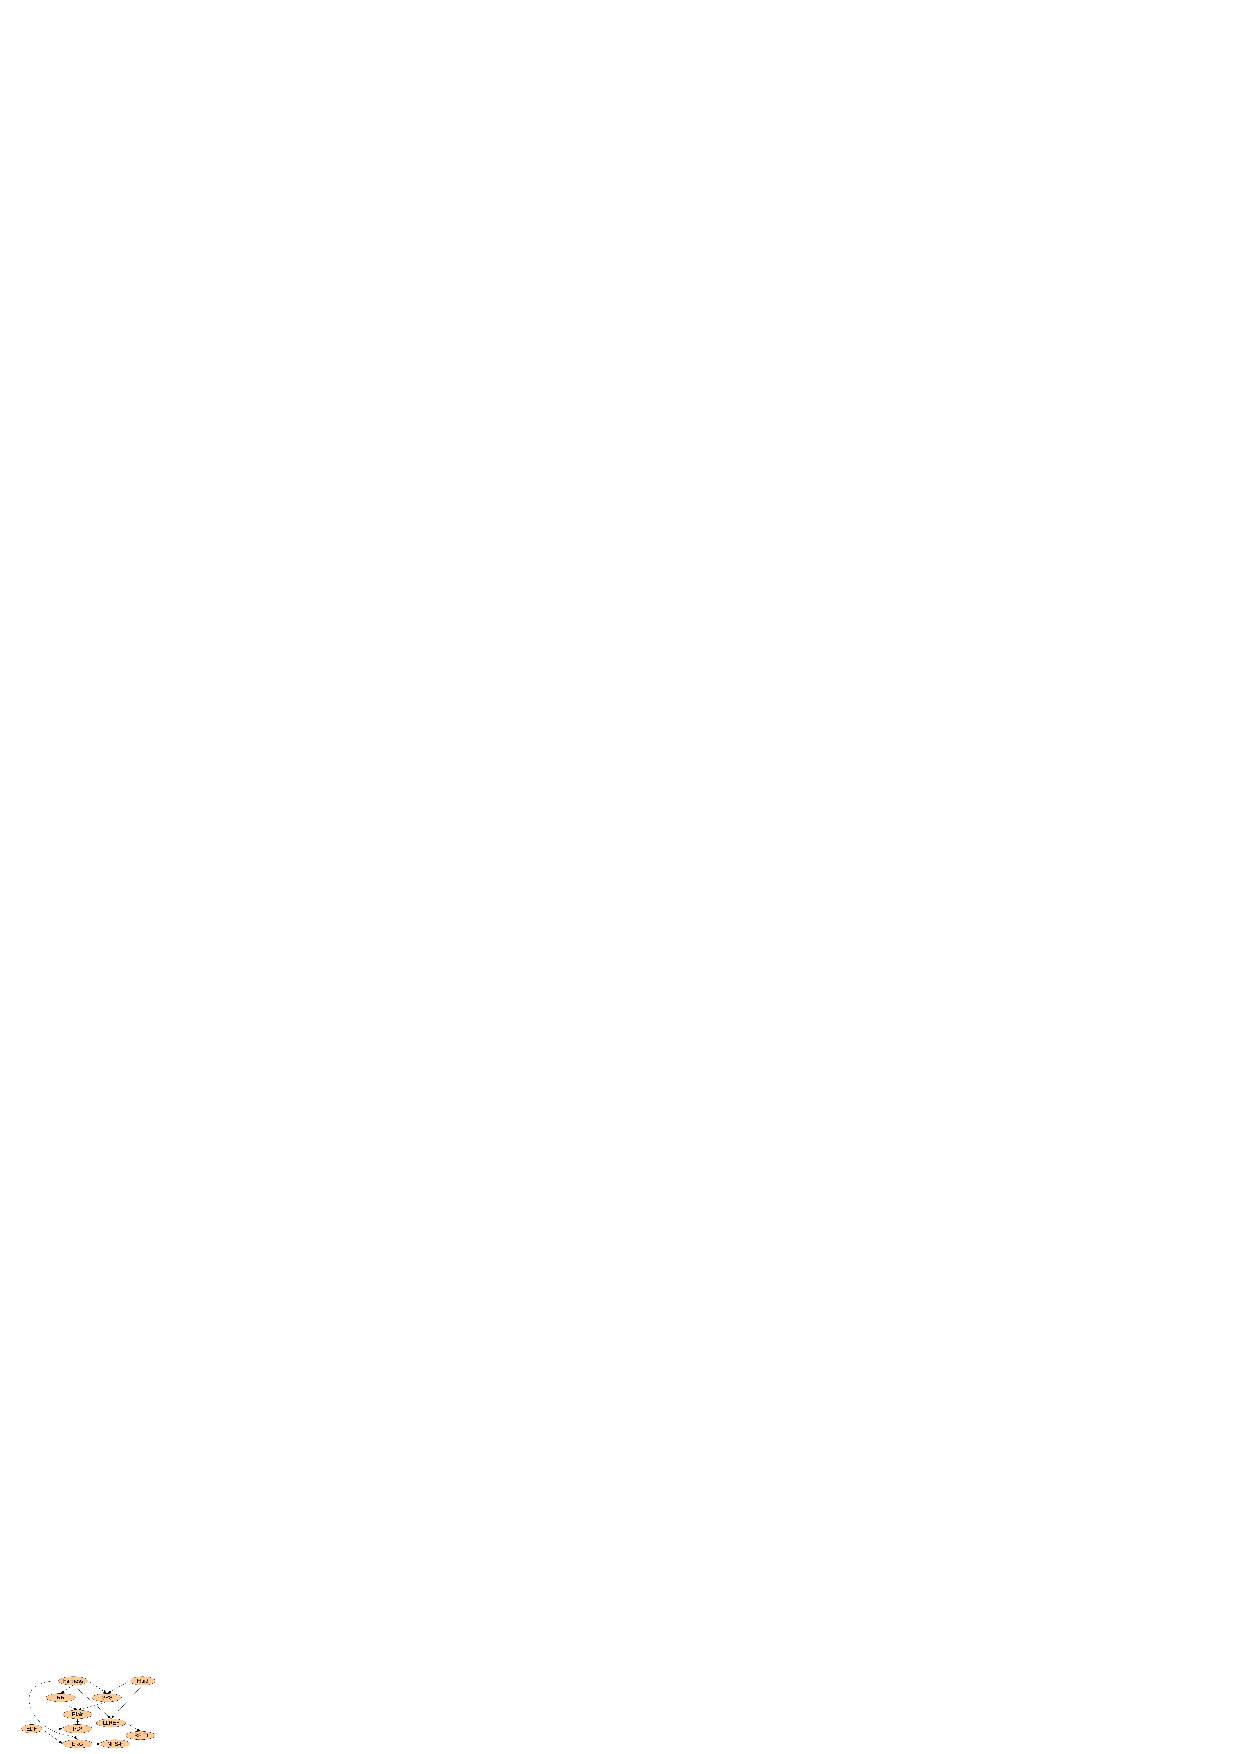
\includegraphics[width=10cm]{img/genealogy_pf}
	\end{figure}
	Ils précisent qu'\textit{EDF} n'est pas concerné par cette classification, mais qu'ayant 
	inspiré certaines approches, il méritait de se trouver sur cette image. 
	Nous invitons le lecteur intéressé par les influences des algorithmes entre eux 
	à prendre connaissance de cet article extrêmement documenté.\medskip
	
	De la lecture des articles, il ressort qu'une partie non négligeable d'entre eux 
	est de parution récente, ce qui montre l'intérêt scientifique actuel pour ce type d'algorithmes. 
	Bien évidemment, les propositions diffèrent par certaines propriétés. Par exemple, 
	\textit{LB-Pfair} est orienté vers les systèmes critiques tolérants aux erreurs. 
	Un enjeu très important de ce grand nombre d'algorithmes est de trouver une méthode qui 
	garantisse l'optimalité pour la classe sporadique, tout en conservant de bonnes performances. 
	
	La préoccupation principale actuelle est de trouver un moyen d'améliorer l'utilisation des processeurs (limitée à 
	50\% pour les algorithmes partitionnés \cite{oh_utilization_1998}), sans détériorer les performances par 
	une explosion du nombre de migrations, comme c'est généralement le cas avec des algorithmes globaux. 
	Dans l'article d'Andersson de 2006 \cite{andersson_multiprocessor_2006}, la limite d'utilisation 
	n'est pas aussi importante qu'avec une approche globale, mais le nombre de préemptions est limité par 
	une constante $k$. En 2006 toujours, Cho et al. \cite{cho_optimal_2006} proposent \textit{LLREF} 
	(largest local remaining execution time), dont l'optimalité est prouvée pour les 
	systèmes périodiques. Ses performances ne sont à ce jour pas bien connues en pratique. 
	La liste proposée ici n'est pas exhaustive, un très grand nombre de propositions existe actuellement. 
	
	\subsection{EDF-k}
	En 2003, Goossens et al. proposent l'algorithme \textit{EDF-k} \cite{goossens_priority-driven_2003}, 
	dont l'idée principale est d'être basé sur la priorité. 
	La définition de \textit{Priority-driven Algorithm} (axé sur les priorités) 
	est donnée par Ha et Liu en 1994 :
	\begin{mydef}
		A Scheduling algorithm is said to be a priority driven scheduling algorithm if and 
		only if it satisfies the condition 
		that for every pair of jobs $J_i$ and $J_j$, if $J_i$ has a higher priority than $J_j$ at 
		some instant in time, then $J_i$ always has higher priority than $J_j$.
	\end{mydef}
	(Un algorithme d'ordonnancement est considéré comme axé sur les priorités si et seulement si il 
	satisfait la condition suivante que pour chaque paire $J_i$ et $J_j$, si $J_i$ a une plus 
	grande priorité que $J_j$ à un instant, $J_i$ a alors toujours une plus grande priorité 
	que $J_j$.)\medskip
	Suivant cette idée, \textit{EDF} est axé sur les priorités, là où \textit{PF} ne l'est pas.\medskip
	
	Reprenant l'idée précédente de \textit{EDF-US} dont certaines tâches étaient de priorité 
	supérieures, et d'autres de priorité simplement assignées par \textit{EDF} "classique", 
	le nombre $k$ représente le nombre stable de tâches ($-1$) concernées par ces priorités 
	supérieures. En d'autres termes, \textit{EDF-k} donne la priorité la plus élevée à 
	$k - 1$ tâches, tandis que les autres sont ordonnancées suivant \textit{EDF}.\medskip
	
	L'article propose une équation dont on dérive la valeur optimale de $k$, et où l'on peut 
	atteindre $m$ le plus petit, cette valeur étant améliorée par rapport à \textit{EDF-US}.\medskip
	
	Une autre approche consiste à considérer la laxité pour modifier \textit{EDF}. 
	Ainsi, l'idée d'\textit{EDZL} (Earliest Deadline until Zero Laxity) \cite{cirinei_edzl_2007} ou encore d'EDCL \cite{kato_real-time_2007}
	(Earliest Deadline Critical Laxity). \medskip
	
	Des travaux récents continuent d'implémenter des versions d'\textit{EDF} avec stratégie 
	globale, par exemple \textit{GEDF} \cite{li_global_2015}, donnant lieu à \textit{PGEDF}. Cette 
	branche continue donc d'être étudiée et présente des intérêts.
	
	\subsection{U-EDF}
	\textit{U-EDF} est présenté en 2011 par Nelissen et al. \cite{nelissen_reducing_2011}. Il n'est pas "\textit{P-Fair}", et se démarque donc d'une bonne partie des algorithmes 
	par le fait qu'il ne cherche pas à vérifier de condition de "P-équité".
	Il prend en charge les systèmes périodiques à échéances implicites, et est optimal pour cette classe. 
	Tout d'abord, la preuve de son optimalité se limite aux tâches périodiques dont on a dit plus haut qu'elles 
	ne représentaient pas la majorité des classes e tâches des systèmes embarqués. 
	En 2012, la preuve de son optimalité est élargie aux systèmes sporadiques par Nelissen et al. \cite{nelissen_u-edf_2012}. Le principal but de cet algorithme est de réduire le nombre de préemptions, 
	ce qui est un grand inconvénient de l'approche globale. \medskip
	
	\subsection{RUN}
	Reduction to UNiprocessor (\textit{RUN}) est un algorithme présenté par Regnier et al. en 2013 \cite{regnier_multiprocessor_2013}. 
	Cet algorithme est appliqué aux systèmes périodiques préemptifs à tâches indépendantes à 
	échéances implicites. \textit{RUN} -- contrairement aux exemples vus précédemment -- n'applique pas 
	la \textit{P-Fairness}, et parvient à réduire significativement le nombre de préemptions. 
	\textit{RUN} réduit un ensemble de tâches en plus petits ensembles plus facilement ordonnançables 
	en suivant deux opérations :\medskip
	\begin{itemize}
		\item Une opération "\textit{Dual}"
		\item Une opération "\textit{Pack}"
	\end{itemize}
	Un \textit{Dual} se construit par complémentarité avec un \textit{Primal}, dont les règles de constructions sont 
	données dans l'article.
	Un serveur est chargé d'ordonnancer chaque sous-système. Celui-ci fonctionne à l'aide 
	d'\textit{EDF}, dont les avantages nombreux ont déjà été évoqués plus tôt dans ce document. 
	Il n'est pas évident à la lecture de l'article de comprendre en quoi 
	diffère l'approche de \textit{RUN} par rapport à un ordonnanceur 
	partitionné qui donnerait lieu à des systèmes ordonnancés à l'aide d'\textit{EDF}. 
	En réalité, \textit{RUN} n'est pas un algorithme global, mais plutôt 
	semi-partitionné, et la différence tient particulièrement du fait que les systèmes ne sont pas 
	gérés par des processeurs distincts mais par des serveurs.  
	Les auteurs insistent sur les avantages théoriques de RUN, qui devraient motiver une implémentation 
	pratique afin de tester ses avantages. Cette implémentation a été faite 
	\cite{compagnin_putting_2014} sur $LITMUS^{RT}$, et dont les résultats demandent à 
	être confirmés mais montrent les bonnes performances sur ce système.\medskip
	
	\textit{RUN} -- malgré son apparition récente -- a déjà des successeurs. \textit{QPS}
	(Quasi Partitioned Scheduling) est un algorithme 
	également semi-partitionné, mais à la différence de RUN, il peut ordonnancer les systèmes de tâches indépendantes sporadiques à échéances implicites. 
	Il est décrit dans un article de Massa et al. \cite{massa_outstanding_2014} en 2014. 
	Comme pour \textit{RUN}, \textit{QPS} génère des sous-ensembles de tâches qui seront ordonnancés 
	selon \textit{EDF} par des serveurs. Les auteurs présentent l'avantage d'une approche semi-partitionnée, 
	qui fait un compromis entre les avantages de l'approche partitionnée et ceux de l'approche globale 
	mais \textit{RUN} comporte quant à lui l'inconvénient de ne pas pouvoir s'appliquer aux tâches sporadiques. C'est ce qui explique la nécessité de l'existence de \textit{QPS}.
	L'avantage de \textit{QPS} est de pouvoir adapter sa stratégie en fonction de la
	charge. En effet, durant le runtime, \textit{QPS} peut s'adapter, passant d'une
	stratégie \textit{globale} à \textit{partitionnée}, ou le contraire. 
	Pour ce faire, \textit{QPS} va diviser les tâches en sous-systèmes, classés différemment selon leur besoin en processeur :\medskip
	\begin{itemize}
		\item \textit{mineur}, si le sous-système a besoin d'un seul processeur
		\item \textit{majeur}, si le sous-système a besoin de plusieurs processeurs
	\end{itemize}
	Par conséquent, si tous les sous-systèmes sont mineurs, \textit{QPS} fonctionne comme 
	\textit{EDF} partitionné. Dans le cas contraire, l'exécution dépendra des besoins 
	des sous-systèmes, et pourra être composé de plusieurs \textit{serveurs QPS} 
	en mode multi-processeur, ou en \textit{EDF} sur simple processeur, cumulant 
	deux modes. \medskip
	Les résultats attendus de \textit{QPS} sont donc très prometteurs, car il permet de 
	conjuguer les avantages des approches partitionnées ainsi que globales.
	
	\subsection{Tableau comparatif des algorithmes globaux et semi-globaux}
	Afin de faire le choix de l'algorithme à implémenter, une comparaison de ces algorithmes 
	devrait être faite afin d'orienter le choix vers un ordonnanceur plutôt qu'un autre. 
	
	\vspace{1em}
	
	\begin{tabular}{|c|c|c|c|}
		\hline
		\customhighlight{Nom} & \customhighlight{Classe} &  \customhighlight{Optimal} & \customhighlight{Migrations}\\
		\hline
		\hline
		EDF-k & Sporadique, échéance implicite & Optimal (P-Fair) & Nombreuses \\
		\hline
		GEDF & Sporadique, échéance implicite & Non optimal & Nombreuses \\
		\hline    
		U-EDF & Sporadique, échéance implicite  & Optimal & Réduites\\
		\hline
		DP-WRAP & Sporadique, échéances arbitraires & Optimal (P-Fair)& Réduites\\
		\hline
		LLREF & Périodique, échéances arbitraires & Optimal & Réduites \\
		\hline
		BF & Périodiques, échéances implicites & Optimal & Réduites \\
		\hline
		RUN & Périodiques, échéances implicites & Optimal & Un peu réduites\\
		\hline
		QPS & Sporadiques, échéances arbitraires & Optimal & Réduites\\
		\hline
		
	\end{tabular}
	\bigskip
	
	\section{Conclusion}
	Nous avons exploré une petite partie de la littérature scientifique au sujet des ordonnanceurs 
	globaux ou semi-partitionnés afin d'en sélectionner un pour implémentation et tests. 
	Il ressort de cette étude que plusieurs candidats présentent des intérêts, sont mieux 
	connus dans la littérature que dans la pratique, et gagneraient à être mieux analysés. 
	Notre choix sera influencé par ces paramètres : \medskip
	\begin{itemize}
		\item L'ordonnanceur est-il optimal
		\item Quels systèmes de tâche peut-il ordonnancer ?
		\item Des efforts ont-ils été fournis afin d'éviter les migrations ?
		\item A-t-il déjà bénéficié d'implémentations ?
	\end{itemize}
	De ces paramètres, il ressort que l'algorithme \textit{QPS} est optimal, semi-partitionné, 
	peut ordonnancer les systèmes sporadiques à échéances arbitraires et 
	les articles à son sujet parlent de bonnes performances concernant les migrations. \medskip
	C'est donc vers cet algorithme que notre choix se porte.
	
	
	\bibliographystyle{plain}
	\bibliography{bibzotero}
	
\end{document}


